\section{Shortcodes}\label{shortcodes}
In diesem Kapitel wird sich den Thema \emph{Shortcode} gewidmet. Dabei wird nach einer kleinen Definition, die Benutzung und der Einsatz in einer Wordpressumgebung erläutert. 
\subsection{Was ist ein Shortcode?}
Um Shortcodes zu verwenden, wird nun erläutert, um was es sich hierbei handelt. Nach Bondari und Griffiths
\footcitetgedr[Vgl.][Seite 177]{BB11} lässt sich ein Shortcode als Makro definieren, welches in einem Artikel oder Seite hinzugefügt werden kann. Damit lassen sich also bestimmte Funktionen zu einer Seite hinzufügen. \newline
Die offizielle technische Dokumentation von Wordpress\footcitetint[Vgl.][]{MMTSA12} bringt des weiteren noch hervor, dass ein Shortcode von einem Pluginentwickler dem eigentlichen Benutzer dabei hilft, auf einer bestimmten Seite - also im Frontend von Wordpress - das Plugin einzubinden.
\subsection{Shortcodes verwenden}
In Abbildung \ref{img:SHISEINB} ist der Shortcode für das Mentoren-Plugin abgebildet, welcher im Inhaltsbereich einer Seite / Artikel das Frontend der Mentorensuche einbindet - und zwar genau an der Stelle, an der er eingebunden wird.
   \begin{figure}[htbp]
	\begin{center}
	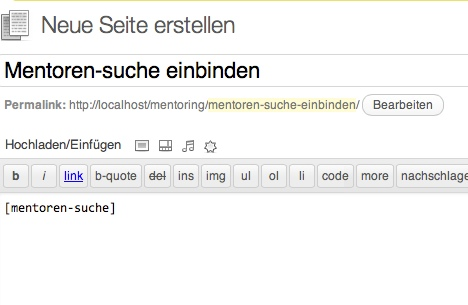
\includegraphics[angle={360}, scale=0.61]{pictures/shortcodeeinb.jpg}
	    \caption{Shortcode in Seite einbinden}
	    \label{img:SHISEINB}
	\end{center}
   \end{figure}\newline
Im Anschluss lässt sich die neue Seite (Abbildung \ref{img:shortcideeinber}) im Browser betrachten:
   \begin{figure}[htbp]
	\begin{center}
	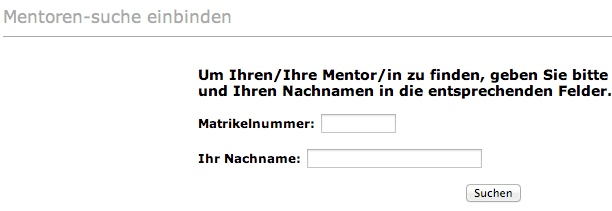
\includegraphics[angle={360}, scale=0.61]{pictures/shortcideeinber.jpg}
	    \caption{Ergebnis des eingebundenen Shortcodes}
	    \label{img:shortcideeinber}
	\end{center}
   \end{figure}
   \newpage
Wie ein solches Frontend erstellt wird, wird näher im Kapitel Formularerstellung (siehe Kapitel \ref{Formular}) erläutert. Hier geht es erstmal um die Einbindung solcher Funktionen.\newline
Schauen wir uns also an dieser Stelle genauer an, wie ein Shortcode erstellt ist. Die allgemeine Syntax ist in Listing \ref{CSHHIN} dargestellt. Der erste Teil beschäftigt sich mit der allgemeinen Syntax, anschließend ist ein Beispiel dargestellt. Dabei sollte diese Funktion in der Hauptdatei des Plugins vorhanden sein. Also beispielsweise \emph{mentoren-suche.php}.
\lstset{language={PHP},caption={Shortcode hinzufügen},label=CSHHIN}
\lstset{
 morekeywords={require_once,add_shortcode}
}
\begin{lstlisting}
<?php
...
// Allgemeine Syntax fuer einen Shortcode
add_shortcode('Shortcodename','AufzurufendeFunktion');
...

// Beispieldefinition des Shortcodes
require_once('frontend.php'); //frontend.php muss vorhanden sein
add_shortcode('mentoren-suche','showSearchArea');
...
?>
\end{lstlisting} 
Festzuhalten ist, dass Shortcodes sich ähnlich zu Filtern verhalten: Es werden Parameter akzeptiert und ein Ergebnis wiedergegeben. Dabei hat die \emph{add\_shortcode}-Funktion zwei Parameter: Einmal den Shortcodename, welcher dann in einem Post eingebunden werden kann (siehe \emph{mentoren-suche} und die aufzurufende Funktion \emph{showSearchArea}.\footcitetint[Vgl.][]{MMTSA12} \newline
an dieser Stelle soll auch ein kleiner Blick auf die Funktion \emph{showSearchArea} geworfen werden, um einen ersten Eindruck der Funktion zu bekommen. Diese ist (gekürzt) in Listing \ref{CSHFUNSSA} dargestellt.
\lstset{language={PHP},caption={Gekürzte Beispielfunktion showSearchArea},label=CSHFUNSSA}
\lstset{
 morekeywords={function,require_once,add_shortcode}
}
\begin{lstlisting}
/**
* Zeigt die Suchmaske fuer das Frontend an.
*/
function showSearchArea()
{ 
  //Variablendefinitionen
  
  if(isset($send_mentorenSearch))
  {
  ...
  		// Ausgabe des Ergebnisses
  		// Fehlermeldung: Eingabedaten sollten vervollstaedigt werden 	
  ... 
 }
 else{
   ...  
     // Eingabe der Matrikelnummer und des Nachnamens
   ...
 }
}
\end{lstlisting} 
Diese Funktion ist in der Datei \emph{frontend.php} vorhanden und dient dazu, ein Formular mit einer Suchfunktion darzustellen.Dabei wird geprüft, ob ein Ergebnis vorliegt - also falls der entsprechende Datensatz gefunden wurde. Falls keiner gefunden wurde, wird eine entsprechende Fehlermeldung ausgegeben. Zusätzlich erfolgt bei einer leeren Eingabe eine Meldung, dass Matrikelnummer und Nachname eingeben werden müssen und ein Link zur Suchformular verweist. Weitere Informationen für Shortcodes finden sich unter \url{http://codex.wordpress.org/Shortcode}. \newline
Im nächsten Kapitel geht es um die Wordpress \nameref{shapi}.
\subsection{Shortcode-API}\label{shapi}
Die Shortcode-\gls{API} wurde mit Wordpress 2.5 eingeführt und beinhaltet Funktionen, um spezielle Makros zum erstellen von Shortcodes in Posts zu verwenden.\newline
An dieser Stelle werden ausgewählte Funktionen vorgestellt und erläutert\footcitetint[Vgl.][]{MMTSA12}:
\begin{enumerate}
	\item {\bf function add\_shortcode(\$tag, \$func)} 
	\begin{itemize}
		\item Diese Funktion wurde bereits im Beispiel-Listing \ref{CSHHIN} verwendet und dient dazu, neue Shortcodefunkionen zu registrieren.
		\item Dabei ist \emph{\$tag} der Shortcodename, welcher der Benutzer in einem Post verwenden kann
		\item Der zweite Parameter \emph{\$func} dient dazu, eine bestimmte Funktion auszuführen, wenn der Shortcode aktiviert wird.
	\end{itemize}
	\item {\bf function remove\_shortcode(\$tag)} 
	\begin{itemize}
		\item Im Allgemeinen lässt sich hiermit ein Shortcode von einer Seite entfernen und es wird nur der Inhalt angezeigt, der auch ohne Shortcode vorhanden ist.
		\item Der Parameter \$tag entspricht hierbei dem Shortcodenamen, der von Benutzer verwendet wird (Parameter 1 in \emph{add\_shortcode})
		\item Beispielsweise lässt sich diese Funktion verwenden, wenn auf einer Seite ein oder mehrere Shortcodes eingebunden sind und eine davon temporär oder für immer deaktiviert werden soll, ohne das entsprechende Plugin zu deinstallieren.
	\end{itemize}
	\item {\bf function remove\_all\_shortcodes()} 
	\begin{itemize}
		\item Diese Funktion deaktiviert im Gegensatz zu \emph{function remove\_shortcode(\$tag)} alle Shortcodes auf einer Seite.
	\end{itemize}
	\item {\bf function do\_shortcode(\$content)} 
	\begin{itemize}
		\item Die Funktion do\_shortcode(\$content) eignet sich dazu, in einem Post andere Funktionen zusätzlich einzubinden. Beispielsweise könnte dies ein Kontaktformular sein.
	\end{itemize}
\end{enumerate}
Weitere Funktionen sind auf der offiziellen Shortcode-API seite von Wordpress zu finden (siehe \url{http://codex.wordpress.org/Shortcode\_API#Function\_reference})
